\documentclass{beamer} 

\usetheme{Pittsburgh}
\usecolortheme{beaver}

\usepackage{dot2texi}
\usepackage{tikz}
\usetikzlibrary{shapes,arrows}
\usepackage{bookmark}
\usepackage{graphicx}
\usepackage{todonotes}

\title{Web Search and the BBC}
\author{Ross Fenning}
\institute{
  Senior Software Engineer
  \\Homepage, Search and Navigation
  \\Future Media
  \\BBC
}
\date{23 May, 2013}

\begin{document}

\begin{frame}[plain]
  \titlepage
\end{frame}

\begin{frame}
  \frametitle{What is BBC Search?}
  \framesubtitle{i.e. What do I work on?}
  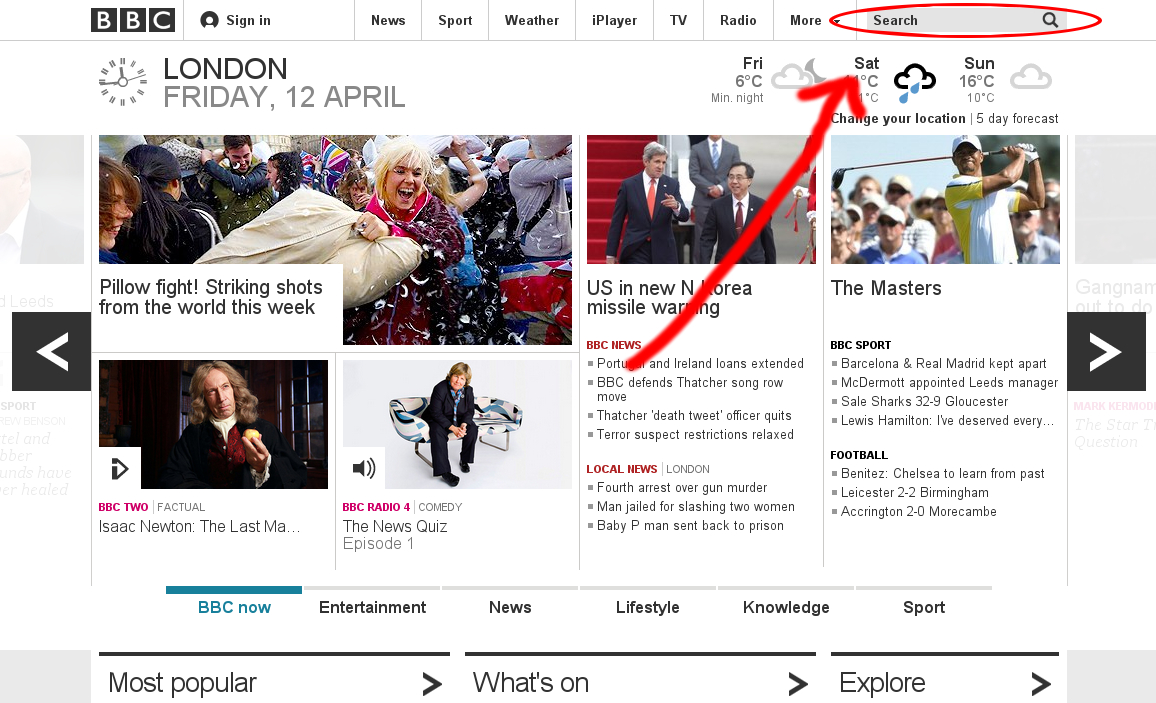
\includegraphics[width=\linewidth]{homepage.png}
\end{frame}
\note{
  I work in the team responsible for BBC's online search facility. The
  first point of entry is usually a the search box on the top right
  as shown. This then takes you to a search results page.
}

\begin{frame}
  \frametitle{BBC Search results}
  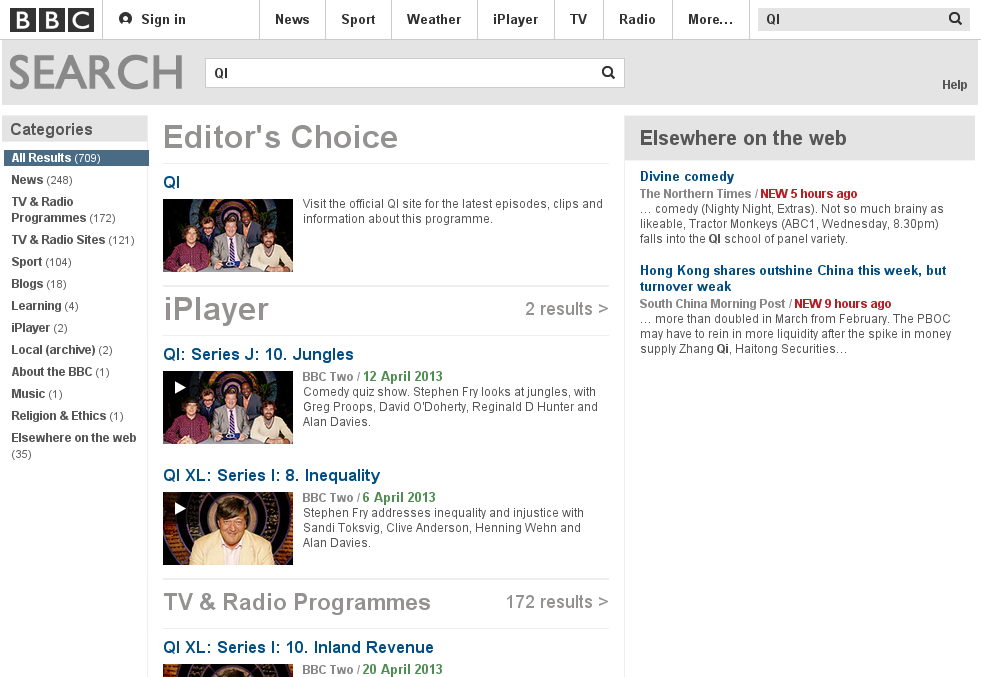
\includegraphics[width=\linewidth]{results.png}
\end{frame}
\note{
  This is the page you get after having done a search if you started
  on the home page as shown previously. You can see the first
  results are chosen by editors as the best results you are likely
  looking for.
}

\begin{frame}
  \frametitle{BBC iPlayer Search results}
  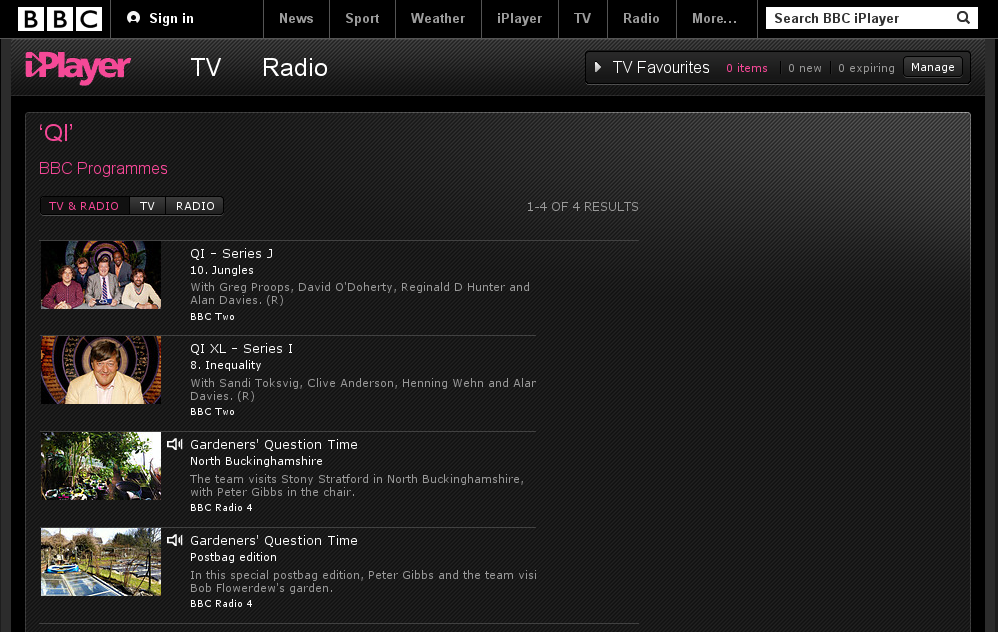
\includegraphics[width=\linewidth]{iplayer.png}
\end{frame}
\note{
  Some parts of the BBC website have a specialised, ``scoped'' search
  that only searches amongst content for that part of the site. Here,
  we see the result of having clicked the ``iPlayer'' navigation link
  and then used the search box.

  This is based on the assumption that if someone is already on the
  iplayer pages, then any searches they do will be for only TV and
  Radio programmes that are currently available to watch or listen to.
}

\begin{frame}
  \frametitle{CBBC Search results}
  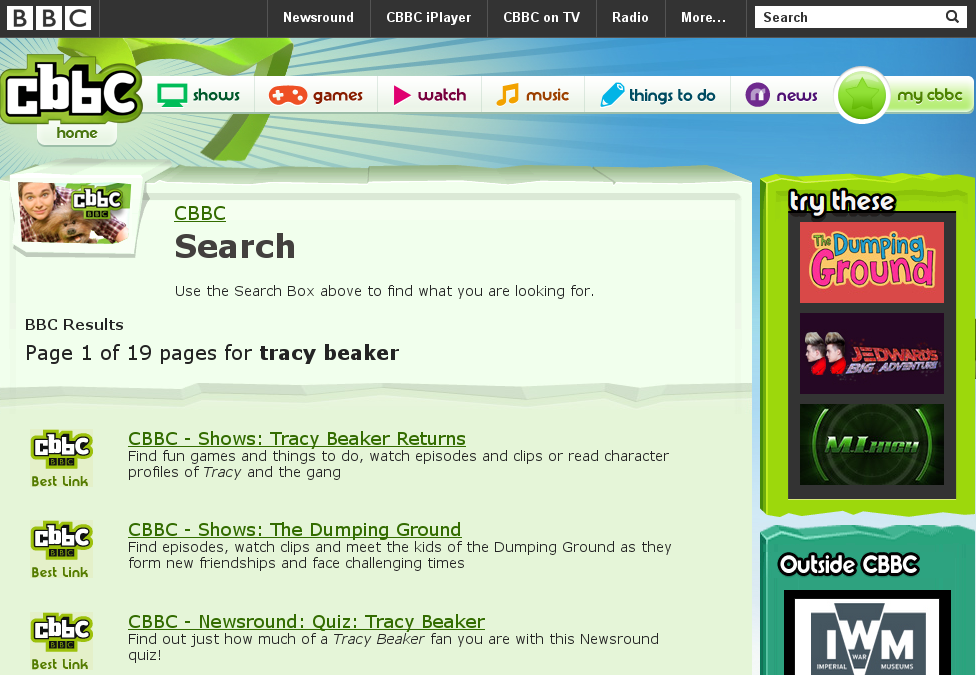
\includegraphics[width=\linewidth]{cbbc.png}
\end{frame}
\note{
  Here, we have a search page that only shows pages and content suitable
  for children under 13. The search scoping is now not just for the
  convenience of only showing pages for the section we're in, but also
  providing a safe, appropriate subsection of the wider BBC website
  for children where they are only navigating, searching and viewing
  things that are known to be suitable.
}

\begin{frame}
  \frametitle{Outline of this talk}
  \begin{enumerate}
    \pause \item What is web search?
    \pause \item Search techniques
    \pause \item Search design patterns
    \pause \item Why does BBC have its own search?
    \pause \item What does the BBC have online?
    \pause \item What does BBC Search look like as software system?
    \pause \item Model-View-Controller (MVC)
    \pause \item Service-Orientated Architecture (SOA)
    \pause \item Event-Driven Architecture (EDA)
    \pause \item How can we index BBC content?
    \pause \item How do we search BBC content?
    \pause \item How can we keep improving the experience?
  \end{enumerate}
\end{frame}
\note{
  Today, I will talk about what web search is academically and generally
  then introduce the ``why'' and the ``what'' of BBC search
  Then we can look at some specific software engineering principles
  relevant to such a large software project and then move on
  to some of the challenges faced by doing a search for the whole of
  BBC online.
}

% Section 1

\begin{frame}
  \frametitle{What is the web?}
  \begin{enumerate}
    \pause \item Collection of pages/documents
    \pause \item Each has a unique address, e.g. http://en.wikipedia.org/wiki/World\_Wide\_Web
    \pause \item Those addresses are known as \emph{Uniform Resource Locators} (URLs)
    \pause \item Pages/documents contain \emph{hyperlinks} to other pages/documents
    \pause \item We now have images, videos, games, etc. and not just pages and documents
  \end{enumerate}
\end{frame}
\note{
  Firstly, it might be useful to outline a precise and distilled
  definition of what the World Wide Web (or WWW or just ``web'')
  actually is.

  The Web is essentially the collection of all pages we can get to
  with a web browser, each with a unique address, known as a
  Uniform Resource Locator or URL. Where the web metaphor
  comes in is that these pages can link to each other by embedding
  each other's URLs and thus pages can reference each other easily.

  Of course, it's not just pages that make up this web, but images
  videos, games, machine-readable information, etc. For a web
  search intended for use by people -- as it the case with Google
  primarily or the BBC Search -- we can focus for now on pages
  (and to some extent videos, games, etc. as people are interested
  in watching and playing those, but they bring their own challenges).
}

\begin{frame}[fragile]
  \frametitle{What is web search?}
  \begin{center}
    \begin{dot2tex}[dot,mathmode,scale=0.8]
      digraph G {
        rankdir=LR;
        node [shape="circle"];
        Crawling -> Indexing -> Querying;
      }
    \end{dot2tex}
  \end{center}
  \begin{enumerate}
    \pause \item Crawl the web to find new pages
    \pause \item Index pages to make it easier to search
    \pause \item Searching/querying the page index
  \end{enumerate}
\end{frame}
\note {
  The process involved in putting together any search engine such
  as Google can essentially be broken down into three phases:
  1) web crawling or otherwise acquiring a list of pages/items that you
  want the search to be able to find; 2) organising those pages/items
  into an index that is easily and quickly searchable; and 3) performing
  searches or queries against that index to present a list of
  pages that are likely of interest to the person who entered a search.

  We can aliken this to creating even a paper index of books within
  a library without even involving a computer-based system. First,
  we must acquire a list of books the library has, which we can do
  by walking along all the shelves and taking note of what we have.
  Then we must take this list of books and organise them in some way.
  For example, we could reorder them into a system such as Dewey Decimal
  where they are grouped by genre or category. We could keep a list
  of which floor of our library has which categories and which books
  we have in each category. We could even
  write some extra keywords on our list next to each book so make it
  easier to see at a glance precisely what each book is about.
  Then, finally we have a visitor who enters the library, tells us
  they are looking for books on, say, psychology and we can refer
  to our list, perhaps ask them to be more specific about their
  query (child psychology, perhaps) and then we can point them
  to a recommended floor, shelf number and possibly a list of book
  titles they might be interested in.
}

\begin{frame}
  \frametitle{Web Crawlers}
  \begin{enumerate}
    \item Visit a page already known about
    \item Add that page to the search index
    \item Find all the links in that page
    \item Store all those links and visit them as well
  \end{enumerate}
\end{frame}
\note {
  A web search such as Google can only know about pages people
  might be looking for by crawling as many pages on the web that
  can be found. This is the equivalent of taking stock and writing
  down all the books on the library shelf, except in this case
  we have a whole web of pages and content that is effectively boundless --
  a stark contrast to a library of very finite size.

  We can start a crawling process by visiting a page we know about -- let's
  say the front page of Wikipedia. We can note the content of that page
  and index it, but the page itself will contain links to many featured articles.
  We can keep a note of all those links, follow them to the articles themselves
  and repeat the crawl process using all the links on those pages.
}

\begin{frame}
  \frametitle{Extracting Content}
  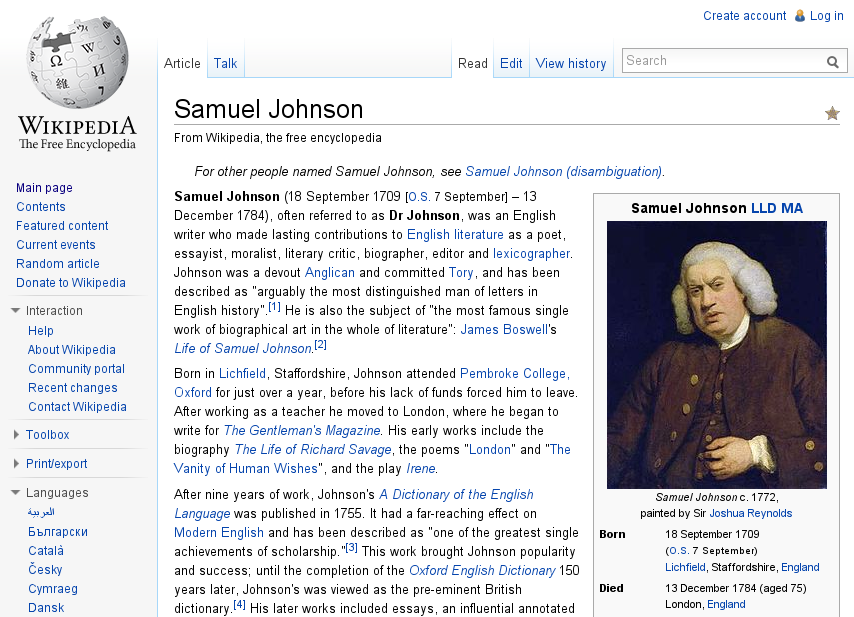
\includegraphics[width=\linewidth]{wikipedia.png}
\end{frame}
\note{
  So, we have a list of pages, like the Wikipedia article shown. Before we
  can create our index, there is at least one important challenge to overcome
  first. Looking at the Wikipedia article shown, there's text that doesn't
  actually form part of the article such as the navigation menu down the side.

  We don't want to suggest this article when someone searches for ``current events''
  or ``random article'', so we need to find a way to identify what is part
  of the actual article and what is not. It's probably clear to us as humans, but
  how do we make a machine understand that distinction? It's less obvious to a
  computer and different websites have different layouts, so this can be quite
  an interesting challenge.
}

\begin{frame}
  \frametitle{Indexing}
  \framesubtitle{e.g. Inverted Index}
  \begin{center}
    \begin{tabular}{|l|l|}
      \hline
      \bf{Documents}   & \bf{Words}             \\ \hline
      Document 1 & three,blind,mice  \\ \hline
      Document 2 & three,little,pigs \\ \hline
      Document 3 & pigs,in,blankets  \\ \hline
    \end{tabular}

    $\downarrow$

    \begin{tabular}{|l|l|}
      \hline
      \bf{Words}     & \bf{Documents}              \\ \hline
      three    & Document 1,Document 2\\ \hline
      pigs     & Document 2,Document 3 \\ \hline
      blind    & Document 1             \\ \hline
      mice     & Document 1             \\ \hline
      little   & Document 2             \\ \hline
      in       & Document 3             \\ \hline
      blankets & Document 3             \\ \hline
    \end{tabular}

  \end{center}
\end{frame}
\note{
  After having crawled or otherwise collected up a collection of documents or
  pages that we might want to present in search results, we need to create
  a search index that will enable accurate and quick queries to be made against
  it. Clearly, reading through every article for keywords entered by a user
  every time a new query in is an inefficient way to work. The process of indexing
  arranges all your documents and pages in such a way as to make searches easier,
  much like the Dewey Decimal categorisation in our library example earlier.

  A very basic form of search index is the \emph{inverted index}. Here, we create
  a lookup table where each word points to the documents that contain that word.
  In the example shown, if a user types in the word ``pigs'', we can point them
  at the second and third document. Note how we can do that with one lookup and
  we are not required to read through each document looking for the word ``pigs'',
  which would be much more time consuming on large documents.

  There are many more sophisticated structures and arrangements that can
  bring other benefits, but this is already a much faster way to find documents
  that match a keyword. However, if we were to add a document that contains
  the word ``mouse'', should that be put in the same row along with the first
  document that contains mouse? This leads us onto the linguistic techniques we
  need to consider when building a search index.
}

\begin{frame}
  \frametitle{Linguistics Techniques}
  \begin{itemize}
    \pause \item Tokenisation
    \begin{itemize}
      \pause \item Breaking sentences up into words or \emph{tokens}
      \pause \item English generally uses spaces, but Chinese does not
      \pause \item \emph{o'clock}? \emph{twenty-one}? \emph{:-)}? \emph{Robin Hood}?
    \end{itemize}
    \pause \item Stemming
    \begin{itemize}
      \pause \item Remove suffixes so that, e.g.  swim and swimming are the same
      \pause \item What's the stem of argue and arguing? Dry and dries?
      \pause \item Overstemming: \emph{Music}, \emph{Musical} and \emph{Musician}
    \end{itemize}
    \pause \item Lemmatisation
    \begin{itemize}
      \pause \item Swim, Swam, Swum
      \pause \item Think, Thought
      \pause \item Good, Better, Best
    \end{itemize}
    \pause \item All of this only applies to \emph{English}
    \pause \item Other languages need their own rules
  \end{itemize}
\end{frame}
\note {
  In the previous slide, we assumed we had already extracted all the words out
  of a document, but even that process might not be as simple as it would seem.
  The process for turning paragraphs of text into individual words or \emph{tokens}
  as the more exact term should be is known as \emph{tokenisation}.

  For English, we can assume a space breaks text into words, but not all languages
  behave this way. Chinese has no boundaries between words. Even in English, we
  sometimes have things like apostrophes or hyphens. Perhaps we might want to
  identify very specific tokens such as smiley faces or maybe we want to treat
  names like \emph{Robin Hood} as a single token since the individual words
  \emph{robin} and \emph{hood} carry very different meanings when encountered
  individually.

  Once we have our words, we probably don't want swim and swimming to be seen
  differently as they are essentially the same word. This is know as \emph{stemming}.
  Stemming gets more complex that just removing letters when you have things like
  \emph{dry} and \emph{dries} where you have to change letters as well as remove
  to get the common stem. Then the problem of \emph{overstemming} can occur when
  removing what looks like simple suffices actually changes the word. Here, we can
  see that \emph{musical} is fine to lose the suffix \emph{-al} where
  it's the adjective from the noun \emph{music}, but it might be incorrect when a document
  is taking about the noun \emph{musical} as in a stage production since those two
  concepts aren't exactly the same thing. It gets worse still if our stemming
  process also decided to reduce \emph{musician} down to the same as music as that
  is, again, a different concept.

  Lemmatisation overlaps somewhat with stemming in that stemming could be seen
  as a na\"ive approach to lemmatisation. Our goal here is not just to reduce
  a word to some root stem before using it for our index, but also to find
  all inflections or variants and reduce them to their \emph{lemma}. So \emph{swimming}
  was previously stemmed to swim, but we also want to recognise that \emph{swam}
  and \emph{swum} could probably be converted to \emph{swim} as well before indexing.
  We have other examples such as think, thought, catch, caught. It's not just verbs
  either as \emph{better} and \emph{best} could be recognised as variants of
  \emph{good}.

  The main difference between stemming and lemmatisation is that stemming happens
  without any real context of the word and can make more mistakes, but is a lot faster.
  Lemmatisation usually takes into account the meaning of the word in the sentence
  and is less likely to confuse things like \emph{musical} the adjective and
  \emph{musical} the noun for a stage production.

  All of this is fairly technical linguistics terminology, but the easiest way to think of
  it all is that the lemma of a word is the form you would look up in a dictionary. So,
  if you wanted to know the meaning of the word ``caught'' you are likely to look
  up ``catch'' and wouldn't really expect there to be an entry for caught.

  The result of this if we look back at our inverted index example before:
}

\begin{frame}
  \frametitle{Stemmed and Lemmatised Index}
  \begin{center}
    \begin{tabular}{|l|l|}
      \hline
      \bf{Words}     & \bf{Documents}              \\ \hline
      three    & Document 1,Document 2\\ \hline
      \bf{pig}     & Document 2,Document 3 \\ \hline
      blind    & Document 1             \\ \hline
      \bf{mouse}     & Document 1             \\ \hline
      little   & Document 2             \\ \hline
      in       & Document 3             \\ \hline
      \bf{blanket} & Document 3             \\ \hline
    \end{tabular}

  \end{center}
\end{frame}
\note{
  We see that our index now prefers the singular forms pig, mouse and blanket. So,
  if we were then to add a document with the word ``mouse'' it would be put in the same
  entry as ``three blind mice'' and a someone querying our search index could
  type ``mouse'' or ``mice'' and it would find either entry. This is clearly
  better for users and you can try this out on Google by searching ``mice'' yourself and
  you will likely get plenty of results with ``mouse'' in the title.
}

\begin{frame}
  \frametitle{Searching the index}
  \begin{itemize}
    \pause \item User enters some keywords
    \pause \item Look up documents/pages that contain keywords
    \pause \item Present a list of results
    \pause \item Should results contain all or just some of the keywords?
    \pause \item What order should results be in?
    \pause \item What other information can be used?
  \end{itemize}
\end{frame}
\note{
  The third and final stage in our search system is the actual searching
  of the index itself. We've already covered this a bit since our
  inverted index made this quite easy with one lookup.

  We start by taking the keywords the user typed in and search our index
  for all documents containing those words and then present a list of
  those documents as candidates for what the user was probably seeking.

  There are many more intricate techniques to do with what to do
  if the document only contains some of the words, how best to order
  the results and Google itself takes into account a lot of contextual
  information such as time and where in the world you are.

  We can look briefly at how we decide which are the better matches so
  we can order the results and also how Google deals with the issue
  of wanting to prefer trustworthy sources for a topic.
}

% Section 2

\begin{frame}
  \frametitle{Scoring}
  \framesubtitle{tf-idf}
  \pause
  \begin{equation}
    \mathrm{tf}(t,d) = \frac{\mathrm{f}(t, d)}{\max\{\mathrm{f}(w, d):w \in d\}}
  \end{equation}
  \vfill
  \pause
  \begin{equation}
    \mathrm{idf}(t, D) =  \log \frac{|D|}{|\{d \in D: t \in d\}|}
  \end{equation}
  \vfill
  \pause
  \begin{equation}
    \mathrm{tfidf}(t,d,D) = \mathrm{tf}(t,d) \times \mathrm{idf}(t, D)
  \end{equation}
\end{frame}
\note{
  So, we've found a list of documents or pages that seem to match
  a search query, but how can we determine which of them is
  the ``best'' match? Searches like Google tend to show results
  as a list from most relevant or best match down to the lesser matches
  towards the end of the list.

  There are many ways to do this, we can look at an example of one
  approach known as \emph{tf-idf}.
}

\begin{frame}
  \frametitle{Google Pagerank}
  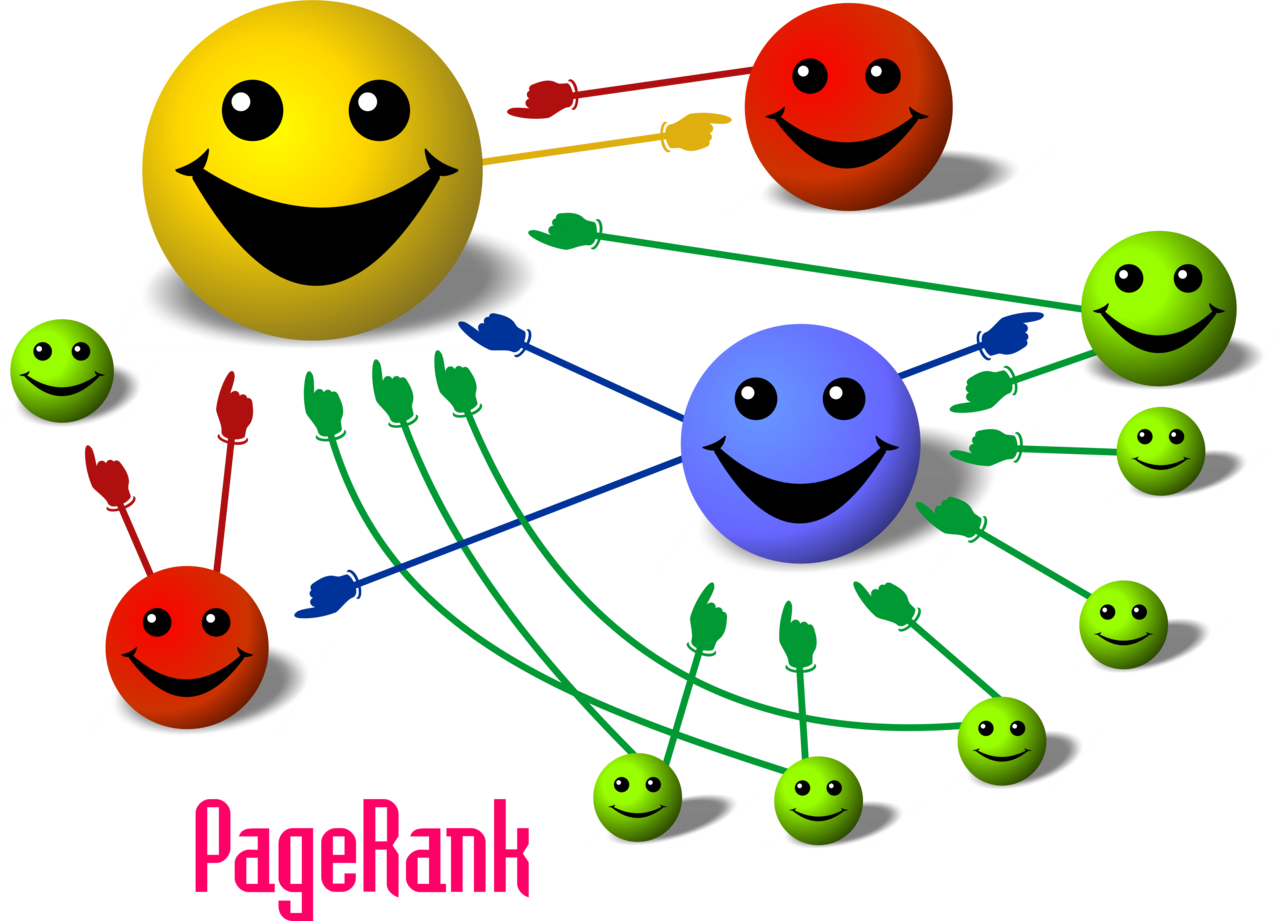
\includegraphics[width=\linewidth]{pagerank.png}\\
  \tiny
  An art draw drawn by Felipe Micaroni Lalli (micaroni@gmail.com).
\end{frame}
\note {
  In the tf-idf scoring algorithm before, we saw that pages and documents
  score highly if they contain many references to a search term, especially
  if that term rarely appears in other documents. The assumption with
  this is that all pages are equal however. This means I can put up
  any old page I like about a topic such as web search and -- if
  I meantion the words web and search enough -- I can appear above
  the Wikipedia article, say, on that topic.

  One disadvantage of
  the World Wide Web is the ease of creating pages allows for a sea
  of non-trustworthy, inaccurate, malicious and unhelpful sites that
  can make finding a reliable and suitable site a difficult endeavour.

  To counter this, Larry Page developed Pagerank at Stanford University
  back in 1996 and this forms a large part of the commercial search
  offered by Google today, although it is likely supported by
  many alterations and additiona algorithms now.

  Briefly, this is best illustrated by the artistic graphic shown here.
  The largest face has the highest Pagerank because it is linked to by
  the most other faces. This is similar to how a lot of people are likely
  to link to well-known and reliable sources such as Wikipedia for general
  topics or BBC News when referring to a current event.

  The smaller faces represent lesser-known sites. They link to other pages,
  but nobody is linking to them, so Google won't give high scores to search
  results unless they are such brilliant matches for a search term that
  they outweigh the larger, well-known sites.

  Note that the red one at the top has only one link to it, yet it is
  larger than the green one nearest it. This is because the link to
  it comes from a very well-respected website and it gives more weight
  to that single link. All Pageranks are calculated in this way in
  that a site with a larger Pagerank feeds more into the Pagerank of
  all other sites it links to. In this way, sites with a lot of respect
  can figuratively ``vouch for'' other sites simply by linking to them.

  Thus the final ``score'' of a potential result for a search query is
  some combination of the keywords in the document and the Pagerank
  notability score.
}

% Section 3

\begin{frame}
  \frametitle{Search Design Patterns}
  
\includegraphics[width=\linewidth]{search_box.png}\\
  \vfill
  \begin{flushright}
    \tiny
    1-02. The iconic search box by Peter Morville\\
    http://www.flickr.com/photos/morville/4273476651/\\
    Attribution-NonCommercial License
  \end{flushright}
\end{frame}
\note{
  So, we've looked at the technical and mathematical side of finding
  content, indexing it for fast retrieval and then performing queries
  against that content index. However a large part of a search application
  is the human interaction with it. Google was notable in the late 1990s
  for its simplistic, no-nonsense interface at a time when other large
  content providers were producing home pages with multiple links
  and other distractions.

  As the web, searching and web design in general has matured over the years,
  common solutions or \emph{patterns} has emerged that we can explore
  briefly now.
}

\begin{frame}
  \frametitle{Standard Search Interface}
  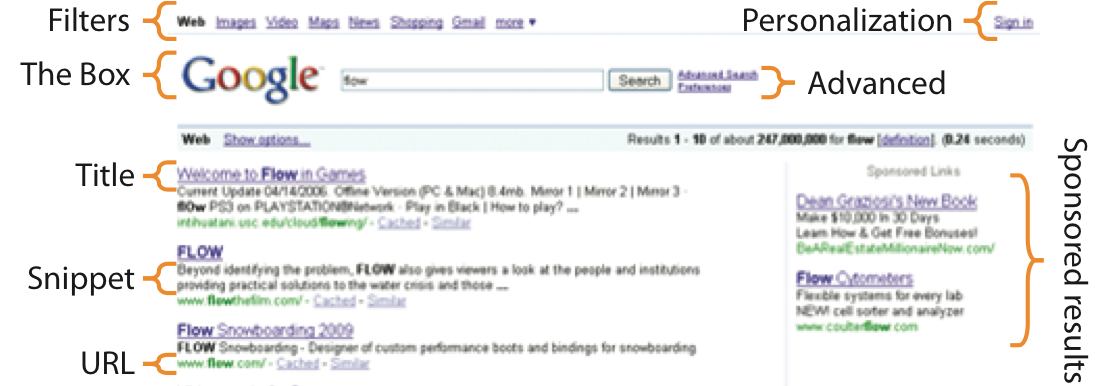
\includegraphics[width=\linewidth]{search_overview.png}\\
  \vfill
  \begin{flushright}
    \tiny
    2-09. Anatomy of a SERP by Peter Morville\\
    http://www.flickr.com/photos/morville/4274260680/\\
    Attribution-NonCommercial License
  \end{flushright}
\end{frame}
\note{
  We can see here the standard search interface common to most search
  systems. There's the search box into which users can type their queries,
  a button such as a magnifying glass for submitting that query and results
  are displayed in a list down the page from ``best'' down to ``worst''
  match.

  So, a common problem with relying on people to type in queries by hand
  is that users don't always write queries that will get the results they
  like. They aren't always aware when they use ambiguous terms, when
  they make spelling mistakes or when they don't give specific enough
  information.

  We can solve some of this in the searching and querying algorithms we
  looked at before. For example, we can make assumptions about what the
  user meant to type if they make a spelling mistake and fix their
  query for them. However, there is only so much you can do before you
  are second guessing the user's intentions and risk the system behaving
  unexpectedly by returning results for a query very different from what
  was actually typed in.

  Since we are looking at design patters, is there a way to solve this
  at the human interface level?
}

\begin{frame}
  \frametitle{Autocomplete}
  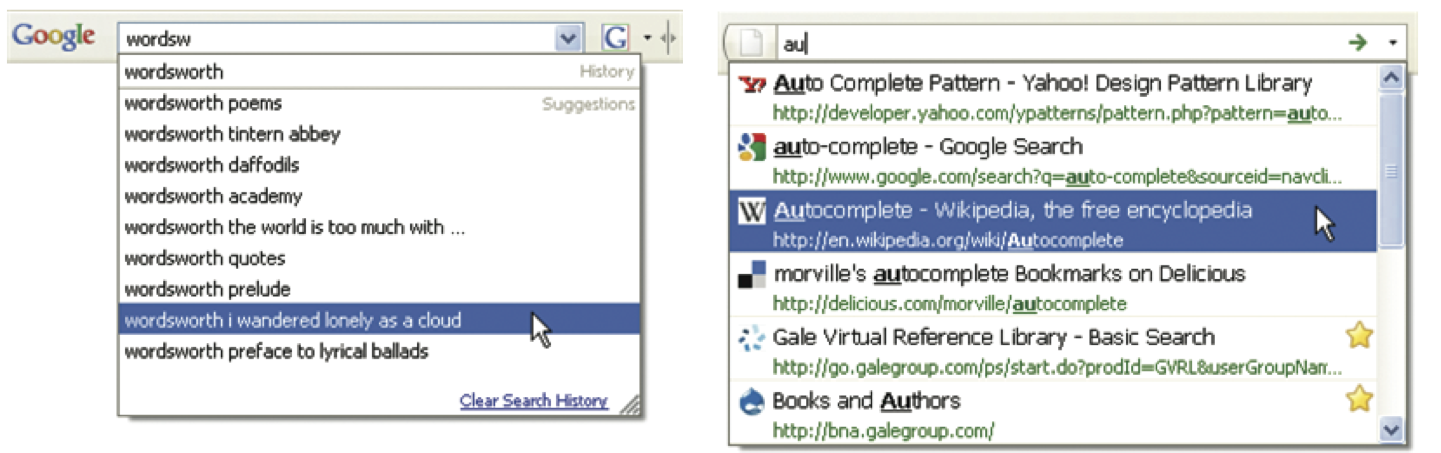
\includegraphics[width=\linewidth]{autocomplete.png}\\
  \vfill
  \begin{flushright}
    \tiny
    4-02. Autocomplete in Google and Firefox by Peter Morville\\
    http://www.flickr.com/photos/morville/4274337384/\\
    Attribution-NonCommercial License
  \end{flushright}
\end{frame}
\note{
  A common feature of search systems is an autocomplete. This is commonly
  implemented as some prompt underneath where you are typing. The prompt
  can suggest words or concepts you might be typing and speed up query
  entry. The side effect of this is that users are more likely to type
  in correctly-spelled words if they choose suggestions more often than
  type them in by hand.
}

\begin{frame}
  \frametitle{Autosuggest}
  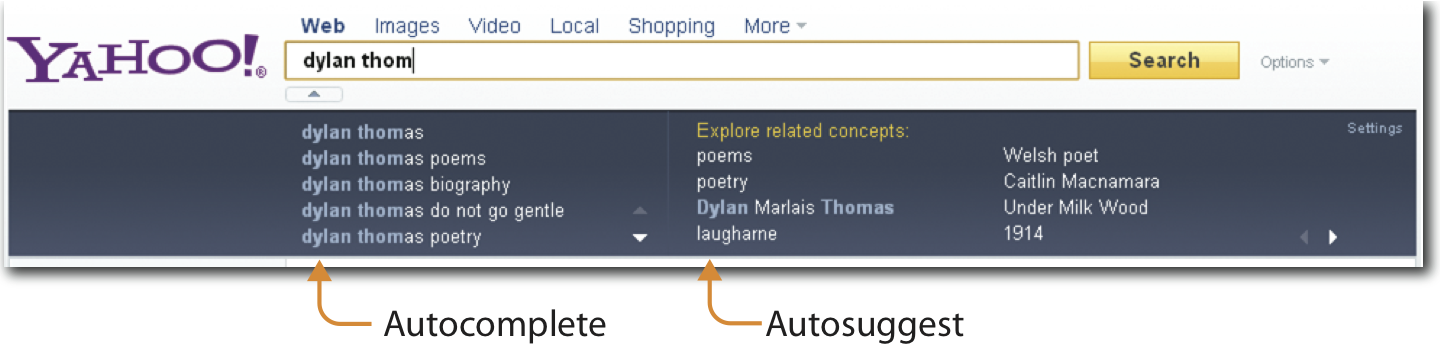
\includegraphics[width=\linewidth]{autosuggest.png}\\
  \vfill
  \begin{flushright}
    \tiny
    4-03. Autocomplete and autosuggest by Peter Morville\\
    http://www.flickr.com/photos/morville/4274337410/\\
    Attribution-NonCommercial License
  \end{flushright}
\end{frame}
\note {
  Autosuggest is a feature similar to, but subtly distinct from autocomplete.
  The mechanism is similar in that a prompt can suggest searches as the user
  is typing their query, but rather than offering potential completions
  of words or phrases in their query alone, more sophisticated and complex
  suggestions can be made.

  For example, we might see that a user is typing in ``what's on TV'' and
  suggest a link to ``TV Schedules''. This is not a completion of what
  the user was typing, but likely a valid suggestion. A user might type
  the number 1 and we might suggest ``BBC One'' or ``BBC Radio One''.
  They might be typing in a football team like ``Manchester U''. We can
  simultaneously offer the completion ``Manchester United'' whilst also
  suggest things like ``Premier League tables''.
}

\begin{frame}
  \frametitle{Spell Check}
  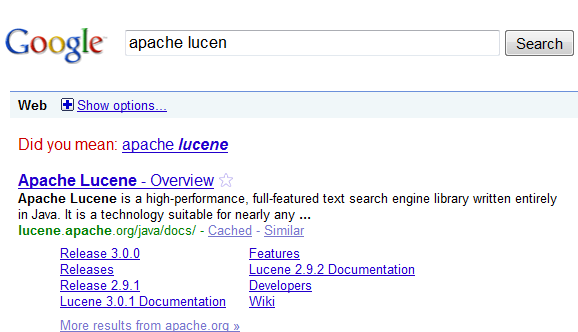
\includegraphics[width=\linewidth]{did_you_mean.png}\\
\end{frame}
\note {
  Another common and recognisable feature for helping users form correct
  queries is one which offers correct spellings of words in their queries.
  More precisely, searches such as Google can offer things like
  ``Did you mean?'' where they can identify that for the sake of changing
  one or two letters, the query would have returned a lot more and better
  results. This does not require a dictionary as such to look up spelling
  mistakes, but more relies on the indexes themselves to be a good
  authority on what are real words or not.

  Google is in a particularly strong position to do such what is essentially
  a statistical approach to correcting search queries. Their indexes are
  perhaps a better record of English (or any language) in its common use
  than any dictionary compiled by hand. They can use this large body
  of real language usage to do their automatic translation service. Instead
  of hiring linguists and translators for every language, they can
  infer a lot based on observations such as whenever an English site
  uses the word ``apple'' a French site tends to use the word ``pomme''.
  Even better is that this gives a contextual sensitivity that a simple
  dictionary could never do. For example, a large collection of French
  and English documents could tell use that ``apple juice'' tends to be
  ``jus de pomme'' in French, but that ``Apple Computers'' tends to be
  exactly the same in French.
}

\begin{frame}
  \frametitle{Facets}
  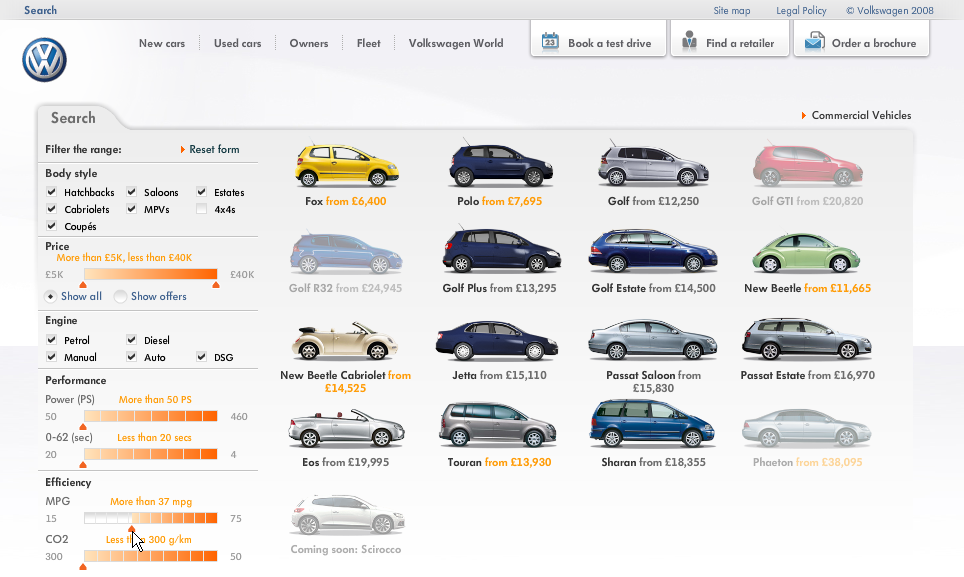
\includegraphics[width=\linewidth]{facets.png}\\
  \begin{flushright}
    \tiny
    Volkswagen UK by Peter Morville\\
    http://www.flickr.com/photos/morville/2367217412/\\
    Attribution-NoDerivs License
  \end{flushright}
\end{frame}
\note{
  Sometimes the results we get back might be quite generic across multiple
  kinds of content. I might enter a generic query such as ``football'' and
  get a mix of football news stories, football results tables, TV programmes
  that feature football and maybe even films that are about football such
  as ``Bend It Like Beckham''.

  A common interface feature here is to provide facets, which are indication
  of the categories your results fall into and allow you to narrow down your
  search to things only within a particular category.
}

\begin{frame}
  \frametitle{Localisation}
  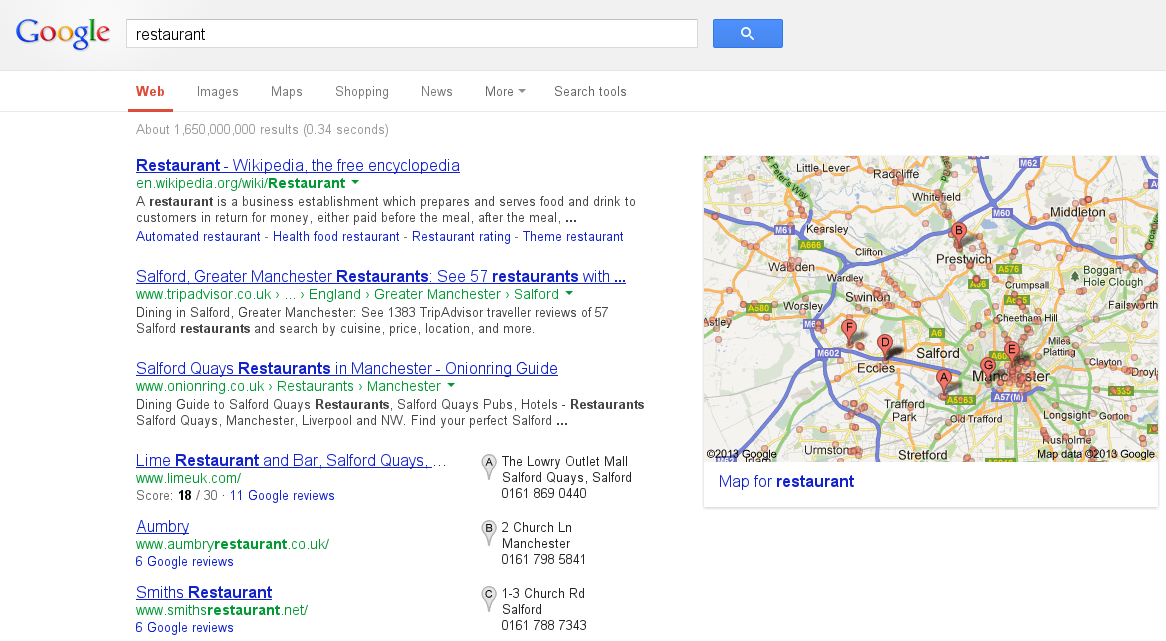
\includegraphics[width=\linewidth]{local_restaurants.png}\\
\end{frame}
\note{
  In all of the search techniques shown so far, what should happen if I search
  ``plumber'' in Google? Clearly any page on the World Wide Web that mentions
  plumber or plumbing is relevant to my search. We can use Google's Pagerank
  to prefer trustworthy sites that receive many links over unknown sites, but
  the obvious problem remains: what use is a very trustworthy plumber in
  Adelaide if I live in Stockport?

  Google already takes your current country into account by virtue of whether
  you are using google.co.uk or google.fr or google.de. This means if we're
  searching for things where the country really matters -- such as local
  businesses -- we can prefer results within the same country. With
  smartphones and other ways of detecting a user's exact location down to city
  or post code level, we can be even smarter and show only plumbers in
  Greater Manchester, say.

  Where can the BBC make use of this? Well, the BBC allows you to search for
  your location already for localising the home page, presenting local
  news or giving you the weather near you. This is something we don't
  currently make much use of, but if a user searches ``local news''
  and we know they live in Cardiff, perhaps we can bias towards news
  local to South Wales?
}

\begin{frame}
  \frametitle{Advanced Search}
  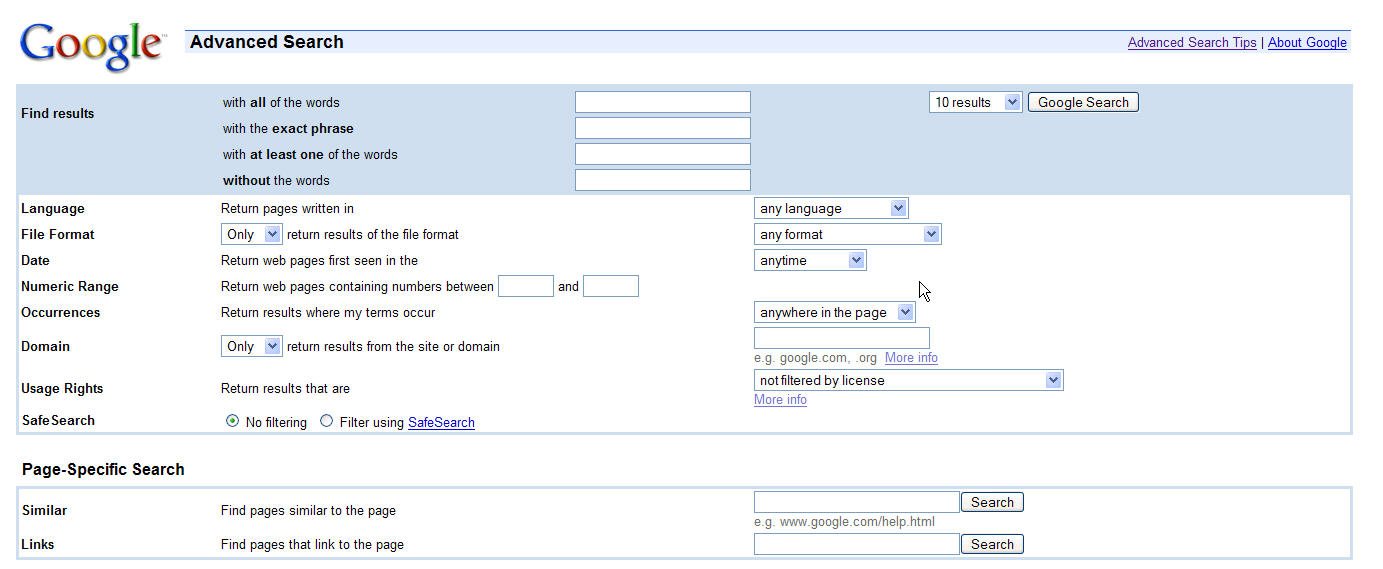
\includegraphics[width=\linewidth]{google_advanced.png}\\
\end{frame}
\note{
  This is a common search feature that might be questionable to the
  average user. Sometimes we want to perform a very exact query for
  a particular search term but with very precise restrictions over
  how recent item is or other aspects such as categories for the items.

  Whilst this can be achieved with facets as shown earlier, a common
  pattern is to allow the user to open up an advanced search form before
  searching anything in order to specify very precise search restrictions.

  The reason why I personally flag it as questionable is that the same
  effect can be achieved by allowing a very basic search in the first
  instance, but then present ways to narrow that down later. A simple
  interface is normally better for most people and Google does not
  even offer ``advanced search'' as a feature. Despite that,
  many other websites offer an ``advanced search'' link that offers
  up a more powerful form for very precise queries.
}

% Section 4

\begin{frame}
  \frametitle{Why BBC Search?}
  \framesubtitle{Isn't Google good enough?}
  \begin{itemize}
    \item We can search the BBC via Google
    \item What can the BBC offer that Google cannot?
    \item Knowledge Graph
    \item BBC Domain Knowledge
  \end{itemize}
\end{frame}
\note{
  So, Google has the ability to search every website on the World Wide Web.
  So, why should a website provide its own search feature? Why, specifically,
  should the BBC provide a search feature?

  Normally, I believe a lot of websites with a lot of text content are
  ill-advised to attempt to build their own search. If they build the site
  in such a way as to be found optimally by the Google crawler, they will
  appear in global searches and Google can also be used to provide
  a local, ``site'' search as well.

  However, Google's text-based indexing and matching doesn't fully
  understand concepts such as BBC programmes, for example. A search on
  Google for ``Question Time'' might just match pages that mention the
  words ``question'' and ``time'' but Google doesn't have the insight
  to know that ``Question Time'' is the exact title of programme produce
  by the BBC.

  Firstly, this is now somewhat misleading in that Google has recently
  released a feature known as ``Knowledge Graph'' in which it attempts to
  understand concepts and present snippets on the side. Secondly, this
  feature still doesn't understand that ``Question Time'' is a concept.
}

\begin{frame}
  \frametitle{Understanding BBC TV Programmes}
  %TODO
  \missingfigure{}
\end{frame}
\note{
  Now, Google results are pretty good when searching for Question Time
  because it's finding pages where those words appear together and
  promoting those to the top of results, but it still lacks some key insight
  the fact that this is a programme and other information about that, such
  as when it is next on or how long it will be available to watch on
  iPlayer.

  The BBC can know that a person is most likely looking for the most
  recent programme, that they might be interesting in similar programmes
  or provide links to information on the actors and characters from
  the show.
}

\begin{frame}
  \frametitle{Understanding BBC Radio Programmes}
  %TODO
  \missingfigure{}
\end{frame}
\note{
  Similarly to understanding TV programmes, we can use knowledge about
  radio programmes.
}

\begin{frame}
  \frametitle{Linking News and other content by topic}
  %TODO
  \missingfigure{}
\end{frame}
\note{
  When someone is searching for the latest news about an ongoing event
  such as the civil war in Syria, we can link news articles based on
  topic and provide links to special pages such as live video streams
  or Q&A overviews.
}

\begin{frame}
  \frametitle{Connecting iPlayer with Learning}
  %TODO
  \missingfigure{}
\end{frame}
\note{
  We can make use of more subtle and sophisticated links between things as
  well. For example, a few years ago an episode of Doctor Who was broadcast
  set in ancient, Roman Pompeii after which there was some increase
  in the number of people searching for information about Pompeii, its
  history and also volcanoes in general.

  Whilst this is not something we're currently doing, but could we perhaps
  be able to add links from the iPlayer page to learning materials related
  to topics brought up in that programme? Could be make better use of
  linking from informational programming such as David's Attenborough's
  Africa or Stargazing Live to all the adult and GCSE learning materials
  on other parts of BBC online?
}

\begin{frame}
  \frametitle{Presenting regional and local information}
  %TODO
  \missingfigure{}
\end{frame}
\note{
  Many companies like Google are vastly improving in the area of giving
  you information and content related to your current location. The rise
  of GPS devices in people's pockets really opens up a lot of opportunity,
  but the BBC has historically always had the remit of providing local
  news, local information and loca weather forecasts to all regions of the
  UK. With the modern web being very focused on the user's current location,
  can the BBC continue to be a leading example with being able to provide
  someone their local weather, travel information and regional news headlines
  all at one as soon as they tell us where they are?
}

\begin{frame}
  \frametitle{Supporting domestic languages}
  %TODO
  \missingfigure{}
\end{frame}
\note{
  And finally, following on slightly from the BBC's obligation to bring
  content and information to the whole of the country, we have the ability
  to focus on searching that information across all domestic languages:
  English, Welsh, Scottish Gaelic and perhaps even Irish Gaelic or Ulster
  Scots. We have a privileged position to cater to the entirety of the UK
  public without being influenced by the commercial drives that back
  English's ability to dominate, largely driven by a US bias in the
  offerings from Silicon Valley. The BBC is not only able to focus on
  catering directly to the British public, but also on areas that US
  companies might well gloss over.

  Of course, the BBC looks internationall as well with World Service and
  BBC Worldwide. We would hope that all search applications and services
  we can develop domestically can go further to support providing World
  Service content in other countries that historically lacked an
  independent press agency and also support the BBC's worldwide, commerical
  efforts.
}

% Section 5

\begin{comment}
  @startuml search_arch.png
  
  skinparam monochrome true
  skinparam componentStyle uml2

  [Web Browser] .d.> () HTTP

  package "Web Application" {
    [Search Results Pages] -u- HTTP
  }


  package "Data Layer" {

    () "Query Interface" as query
    () "Index Entrypoint" as entry
    () "Index Interface" as index

    [Search Results Pages] .d.> query
    [Search Indexes] -u- query

    [Search Indexes] -l- index
    [Transformation Processes] .r.> index

    [Transformation Processes] -u- entry

  }

  package "BBC Content Areas" {

    [News Articles] ..> entry
    [Programmes Information] ..> entry
    [Sport Articles] ..> entry
    [Blog Posts] ..> entry

  }


  @enduml
\end{comment}
\begin{frame}
  \frametitle{What does BBC Search look like?}
  \includegraphics[width=\linewidth]{search_arch.png}\\
\end{frame}
\note{
  So, we have here a very, very abstract view of what a BBC search could look like. It oversimplifies
  some aspects, but it gives a general overview of the approach to architecting an application
  like this.

  At the top we have a user's web browser. So the user is using Firefox, Safari, Internet Explorer, etc.
  to interact with the BBC website and use the search pages. Those search results pages are served
  by what is essentially the web application component. This is the part where the web developers
  and designers work on the interface that the users will see, making the design as effective as
  possible.

  This application does not generate what those results are itself, but relies on calling
  the search indexes through some kind of querying interface. In this way the web application
  acts as a middle man that captures the search queries the user types into their web browser, hands them
  off to the core search engine and then presents the results that come back in a way that's presented
  as appropriately as possible for humans to read.

  This is an example of the principle of \emph{separation of concerns} in software architecture. We
  create separate applications to act as the search engine and the web application responsible for
  interaction with users as they are distinct responsibilities or concerns.

  Modular approaches
  like this in software engineering mean, for example, we can create very different applications
  further down the line that talk directly to the query interface and do very different things
  with the search results. This could be a mobile app that provides a very different interface to
  the main web site or another application altogether that uses the search engine as a data source,
 but does very different things with the information. We don't always know what new features and
  behaviours we will want to add to our software systems at a later date, so a modular approach
  allows us to plug in new components as and when new requirements come up.

  There is another component here that represents the transformation process pipeline that needs
  to happen before items are sent to be indexed. This is grossly understating just how complex
  this currently is -- and perhaps it may always remain complex due to the diverse nature of
  BBC content -- but generalises the need to perform some alteration to content items before
  sending them to the search engine indexes.

  Clearly, a news article looks very different to a TV programme which is again very different
  to a game aimed at children. These are all represented in respective data stores in
  very different ways, but the search indexes need to understand what key words to use,
  what the title of the item is and so on. There is much complex work in ensuring that very diverse
  items like these all enter the search index in some common format and this can involve
  several different applications all communicating over networks.

  We will look at common architectural approaches for very complex applications, but first we will
  focus on the design of the web application side. We can see here that we can group all
  the search indexing and transformation applications into a data layer. In this way, we can
  pretend for the moment that this very complex part of the whole search ecosystem -- which is
  arguably a good 90-odd percent of the complexity -- is a standard data base. In some ways,
  it has a lot of equivalence to a database: it stores information, there is an interface or
  method by which we can put data into it and there is an interface for sending queries
  to get particular subsets of that data later on.

  So, pretending this is just a database and the search results pages are a standard, modern
  web application, what exactly is a standard web application?
}

% Section 6

\begin{frame}
  \frametitle{Model-View-Controller (MVC)}
  \centering
  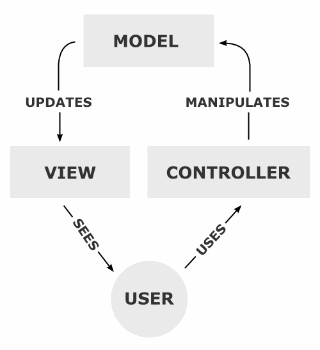
\includegraphics[width=3in]{mvc.png}\\
\end{frame}
\note {
  Stepping back a bit to the general case of most web applications, a common software
  architecture pattern is the so-called MVC or \emph{Model-View-Controller} pattern.

  What is done here is to design some application code that represents the data
  the application will use and name that the \emph{model}. This module or component
  of a web application will provide an interface for other parts of the application
  to retrieve data and manipulate it.

  So, in a search application this could be the component that interfaces with the
  search index itself and provides a way to send search queries to the indexes.

  The part that actually receives requests from a user's web browser is known as
  the \emph{controller}. In a web application, this component is responsible for
  taking requests like submissions of forms or links that are clicked and turn
  them into appropriate interactions with the model component. Again, in our
  search application this may receive the fact that a user typed into a search
  box on the website and pass that query to the model layer so it can send it
  on to the search indexes.

  This, in some ways, acts as a translation between
  the Hypertext Transfer Protocol (HTTP) of the web and the model layer whilst
  also providing
  the ability to catch obvious problems such as the user having failed to type
  in any text at all. The benefit of this separation of concerns again is that
  the model component can be built in such a way that it doesn't concern itself
  with what the web is or who interacts with it. So, if we had a need later on
  to provide, say, a desktop search application that doesn't involve the web
  at all, we can \emph{reuse} the code for the model component that interacts
  with the search indexes and create different desktop application code
  that uses it. Code \emph{reuse} is a very desirable goal in modular software
  design and engineering.

  The last component here is the \emph{view} which is essentially just how
  the information is presented to the user. In our case, search results
  are presented as a single web page listing all the results with titles,
  perhaps thumbnail icons, links and so on. When the user then interacts with
  things like links in that view, those interaction requests are passed back
  around to the controller.

  The view is then the part that the designers can tweak to be aesthetically
  pleasing and user-friendly.

  Note that in our search application, the controller is only asking the model
  for results and doesn't alter the search indexes in any way. In a general
  web application, such as Wikipedia, users can send requests to read and also
  edit the data. This is not impossible for our search application as Google
  provides buttons for people to ``plus one'' results that they felt were
  relevant and thus improve searches for other people. In our MVC architecture,
  such ``plus one'' or ``like'' requests would also go to the controller, who
  then passes these interactions to the model, who will then send requests
  to update the indexes with the popularity of those items.

  One other concern of the controller, is that it might be able to take on
  the role of storing the results of interactions with the model in a
  temporary cache. With this, the controller can hold off bothering with the
  model for the same, popular searches over and over again (e.g. the search
  for Doctor Who now and again in 2 seconds by someone else is unlikely to
  yield different results) and instead simply return a copy of the same view
  shown to the last user to do the same search. Such approaches are essential
  for any application with the significant amount of traffic the BBC gets.
}

\begin{comment}
  @startuml many_databases.png
  
  skinparam monochrome true
  skinparam componentStyle uml2

  [News Website] .d.> [News Database]
  [iPlayer Website] .d.> [iPlayer Database]
  [Nature Website] .d.> [Nature Database]
  [Nature Website] .d.> [iPlayer Database]

  @enduml
\end{comment}
\begin{frame}
  \frametitle{Too many databases}
  \centering
  \includegraphics[width=\linewidth]{many_databases.png}\\
\end{frame}
\note{
  The MVC architecture has become so common that an organisation such
  as the BBC will end up with multiple applications all built in this way
  each with their own model, controller and view. This is fine for someone
  building a small, single-purpose application for their business, but things
  get complicated when we want things to share information across these applications.

  So, again to simplify things quite a bit, we can consider a situation where
  BBC News is its own MVC application, iPlayer is its own MVC application,
  BBC Weather is its own MVC application and so on. This is not the full picture,
  but it illustrates the problem clearly.

  This suggests that news has a ``news'' databases and iPlayer has its own
  database of programmes available to watch. So, if BBC Nature has its own
  database of animals, plants, etc. where does it store information about
  programmes you can watch on iPlayer related to nature? The options seem
  to be that the nature database takes regular copies of all nature
  programmes from iPlayer's database or that the BBC Nature web application
  model component can send queries to both the nature database and the
  iPlayer database at the same time and present the information combined
  in however way it likes.

  So, if we take the first option, we have a situation where there are
  technically two copies of every nature programme's information. One copy
  lives in the iPlayer database and one in the Nature database. There are
  many reasons why duplicating data like this is problematic -- which could
  probably be a whole talk in itself -- but the simplest problem is that
  iPlayer decide to correct something small like a spelling mistake in 
  a programme's synopsis, the Nature site might have a delay before it
  receives the correction. Even worse, what if the process that is copying
  the information stops working one day?

  Modern software architecture tends to prefer to prevent synchronisation
  problems from happening at all rather than constantly working around
  the potential issues, so let's explore the second option where the BBC
  Nature website has direct access to the iPlayer database itself.

  The problems that arise here is now the iPlayer web developers cannot
  restructure their database in any way without remembering to tell
  the team working on BBC Nature, otherwise the BBC Nature web application
  might be left trying to query database tables that no longer exist.

  When one software system is unable to change without another one breaking,
  we can call this a \emph{coupling} problem in that the two systems
  are too \emph{tightly} coupled to each other. If the iPlayer team have to
  keep a list of everyone who is using their database so they can remember
  to tell them when they wish to change it, then they are clearly going to
  be held back from making large changes to the iPlayer web application, which
  is not good for anyone.

}

\begin{comment}
  @startuml service_layer.png
  
  skinparam monochrome true
  skinparam componentStyle uml2

  [Web Application] ..> [Service]
  [Service] ..> [Database]

  @enduml
\end{comment}
\begin{frame}
  \frametitle{``Service Layer''}
  \centering
  \includegraphics[width=1.5in]{service_layer.png}\\
\end{frame}
\note{
  Large organisations like the BBC are more likely to structure their web
  applications like this. The web application itself responsible for
  displaying pages and providing interaction for users communicates over
  a network to another application known as a \emph{service}. These
  service applications only provide data and information in a format
  that can be read and interpreted by the web application, which in
  turn displays that information.

  This back end application can get its information from a database,
  but the key advantage is that the web application doesn't need to
  be concerned with details like that. All we need to ensure is
  that the web application has an agreed way to communicate to the
  service application and we have decoupled the user-facing web
  application from the databases.
}

% Section 8

\begin{comment}
  @startuml service_crosstalk.png
  
  skinparam monochrome true
  skinparam componentStyle uml2

  [News Website] .d.> [News Service]
  [News Service] .d.> [News Database]

  [iPlayer Website] .d.> [iPlayer Service]
  [iPlayer Service] .d.> [iPlayer Database]

  [Nature Website] .d.> [Nature Service]
  [Nature Service] .r.> [iPlayer Service]
  [Nature Service] .d.> [Nature Database]

  @enduml
\end{comment}
\begin{frame}
  \frametitle{Services can communicate with each other}
  \centering
  \includegraphics[width=\linewidth]{service_crosstalk.png}\\
\end{frame}
\note{
  Where we really see the benefit is if we revisit the example
  set of BBC websites from earlier. BBC Nature can use the
  iPlayer service application to pull out any information it needs
  about nature programming it could offer to visitors. The
  iPlayer team are free to change their database any way they see fit
  without fear of disrupting the BBC Nature website so long as
  the iPlayer service keeps providing the specific interface
  they needed.
}

\begin{frame}[fragile]
  \frametitle{Service Orientated Architecture}
  \framesubtitle{Modularity and distributed computing}
  Hypotheical illustration of SOA:
  \begin{center}
    \begin{dot2tex}[dot,mathmode,scale=0.8]
      digraph G {
        rankdir=TB;
        node [shape="circle"];
        "Ecommerce Website" -> Products
        Products -> "Stock Levels"
        "Ecommerce Website" -> Orders
        Orders -> Payments
        "Ecommerce Website" -> "Accounts"
        "Accounts" -> Orders
        Orders -> "Email Confirmation"
      }
    \end{dot2tex}
  \end{center}
\end{frame}
\note{
  What we're starting to head towards is the concept of
  \emph{Service Oriented Architecture} or \emph{SOA}.
  Very briefly, this is an architectural approach for building
  large and complex software systems where what is actually
  developed is a number of individual applications each performing
  a single task only. The complexity of the system is then manifested
  in the interoperation of these components.

  In this simple example, we have an e-commerce website or online shop.
  The website itself needs to query the products service to search
  for products the shop has in its catalogue. It also queries a separate
  stock levels application to get the latest stock count for each
  product it displays. The website can also query the accounts service
  to let a user view or change their details such as card numbers or
  addresses. The accounts service queries the order database so it can
  provide the website with that customer's order information as well.

  The website sends orders the user has completed to the orders service,
  which in turn uses the payments service to determine if the order
  payment goes through. It then uses the email confirmation service to
  send an email to the customer. The email confirmation service perhaps
  even goes back to the accounts service to find the customer's email address
  so it knows where to send the email.

  These principles can be useful for a complex application such as
  indexing all the BBC's online content for search. We have many different
  services that already exist to access that content, but we need a series
  of specific services that can pull in that content when it changes,
  do any conversion, transformations or enhancements and then send it to 
  the search indexes.
}

\begin{frame}
  \frametitle{Information feeds have to be polled}
  \framesubtitle{Or the information producer needs a list of consumers to notify}
  %TODO
  \missingfigure{}
\end{frame}
\note{
  So, we can poll, say, an iPlayer service application to see what programmes
  have been added recently, what's appearing on TV soon and what's newly
  available to watch on catch-up. We can query it, say, every 5 minutes and
  send through any changes from the last five minutes into the search indexes.

  The drawback to regularly polling like this is that there is already a five
  minute delay between something becomming available and when someone
  can actually find it via a search. We could try to reduce this by polling
  every minute, but then we might find the majority of polls come back with
  ``nothing new yet'' as a response. This could be a little inefficient if
  we're sending traffic over a network with no new information. How much
  traffic would be used if we were polling a hundred places every minute?

  An obvious solution to this is to get the source application -- in our
  example the iPlayer service -- to come and tell us when something has changed.
  This means programming a feature into the iPlayer service such that
  whenever it sees a new programme added, it sends a message over to some
  search service application to keep us in the loop.

  A problem with this is iPlayer might end up with 10, 20 or more other
  applications that also want to be notified of changes. What happens
  if the search service is broken and iPlayer is unable to send us the message?
  Does their application fail because of a problem with ours? It seems
  like the iPlayer service is spending more time being concerned about
  whether everyone else is getting the messages rather than focus on its
  own job of showing catch-up programmes to users, which is its primary goal.

  This is again showing signs of tight coupling between the iPlayer service and
  other services.

  Can we do this in a more elegant a clean way?
}

% Section 9

\begin{frame}
  \frametitle{Events}
  %TODO
  \missingfigure{}
\end{frame}
\note{
  Another approach to large software systems that evolves somewhat out
  of service oriented archicture is based around the idea of an
  \emph{event}. The term event here refers to the abstract idea
  that \emph{something is happened} and moreover it is likely some part
  of the system as a whole is interested in being told when that event
  happens.

  So, to go back to iPlayer as an example, the fact a new programme has
  become available for watching on catch-up could be seen as one kind
  of event. Instead of the iPlayer service having to send messages to
  everyone interested in that event, a better approach could be if
  they have some way with which they can simply announce or publish the
  fact that this event has happened. Then if someone is interested in
  knowing when programmes become available, for example the search
  indexes, they can listen out for those announcements or subscribe to
  them in some way.

  This is not too dissimilar to following someone on Twitter or subscribing
  to a blog on the web. A user of Twitter can post a message (or Tweet)
  without specifically being concerned with ensuring it gets to everyone
  and people that have chosen to follow that user will see that message
  appear in front of them. If you want to receive updates from a particular
  person, you follow them, if you do not want to hear from them, you cease
  following them. This is entirely in the hands of the receiver of the message
  and doesn't require either constantly watching/polling someone's messages
  nor the publisher having to go through a list of all subscribers and send
  them the message directly.
}

\begin{frame}
  \frametitle{Event-Driven Architecture}
  %TODO
  \missingfigure{}
\end{frame}
\note{
  The concept of events, systems that publish them and systems that subscribe
  to them is known as \emph{Event-driven Architecture} or EDA.

  Event-driven systems can be as simple sa a burgular alarm where a sensor
  raise an event that a window is open or that movement is detected and
  the alarm component listens for those events and raises an alarm if wishes.

  In the context of indexing BBC online content, we could have a system
  where iPlayer, News, Sport, Nature, GCSE Bitesize, CBBC, CBeebies and
  everyone else raises an event when any information is added, changed
  or removed from their respective websites. Our search application system
  could subscribe to all of those events and update the search indexes
  where appropriate. This is a very idealised view of how an organisation
  with a lot of content could work and in reality every system differs and
  this will not always be possible, but the principles are certainly
  beneficial if applied in the right places.

  The greatest benefit of EDA is that if one service simply publishes
  events of interest for zero, one or many subscribers to follow, but
  without knowing who those subscribers are, then we have achieved truly
  decoupled applications. The iPlayer service can publish the event to
  say that something has changed then get back to working on its
  primary function. It is not burdened with other services that also
  want that information nor affected if those services break in any way.

  It is then our responsibility to build search applications that follow
  those events of changes across all BBC content and design them in such
  a way that if our system does fail in any way, it can pick up where it
  left off when we get it working again -- much like catching up on email
  or your Twitter feed if you've been away for a while.
}

% Section 1

\begin{frame}[fragile]
  \frametitle{What could BBC Search service layer look like?}
  Example view of BBC Search index service applications:
  \begin{center}
    \begin{dot2tex}[dot,mathmode,scale=0.8]
      digraph G {
        rankdir=LR;
        node [shape="circle"];
        News -> "CMS A"
        Sport -> "CMS A"
        CBBC -> "CMS B"
        CBeebies -> "CMS B"
        Programmes -> "CMS B"
        Programmes -> "CMS C"
        "CMS A" -> "Search Entry Point A"
        "CMS B" -> "Search Entry Point B"
        "CMS C" -> "Search Entry Point C"
        "Search Entry Point A" -> "Transformer A"
        "Search Entry Point B" -> "Transformer B"
        "Search Entry Point C" -> "Transformer C"
        "External Information" -> "Transformer A"
        "Transformer A" -> "Search Indexer"
        "Transformer B" -> "Search Indexer"
        "Transformer C" -> "Search Indexer"
      }
    \end{dot2tex}
  \end{center}
\end{frame}
\note{
  So, briefly we can see an overview of how we can multiple services
  applications aggregating content from all over the BBC such that all
  of it ends up on the search indexes so that visitors can search for any
  of them.

  Each of the different areas of BBC online put their information into
  different \emph{content manangement systems} or CMSes. These are
  essentially databases and applications dedicated to storing and managing
  content for people such as articles, videos, images, etc. Some BBC websites
  share the same system for storing their content and some use different ones.
  A lot of the variation is due to the number of years behind each of these
  projects working separately and not necessarily for functional reasons. The
  recent view is to get as much as possible into the same storage location, but
  this is not something that will happen overnight.

  So, for each location where there might be content worth surfacing in
  search results, we need some entry point where that content enters
  the search indexing application. I've given them generic names here, but
  this could be the search application pollng for changes as described earlier
  or that CMS publishing an event of that change.

  The content is going to come out of each system in that systems format,
  which is likey going to need some transformation to convert it to the
  format we need for search and finally it all gets sent into the common
  search indexes.

  This is a simplistic view. The transformation for CMS C, say, might be
  very simple, but the transformation for CMS A could involve a lot of
  further services. Note that I've shown here some external information
  from another source that could be fed into the transformation of items
  from CMS A, which perhaps could enhance the item further. An example of this
  could be that while a News article tells us it's Barack Obama, we might
  then look up in some resource for further information around Barack Obama
  -- perhaps synonyms such as American President -- so we can allow people
  to search using that extra information and not what was literally
  within the article itself.
}

\begin{frame}
  \frametitle{Indexing programmes information}
  \framesubtitle{Structured data}
  \centering
  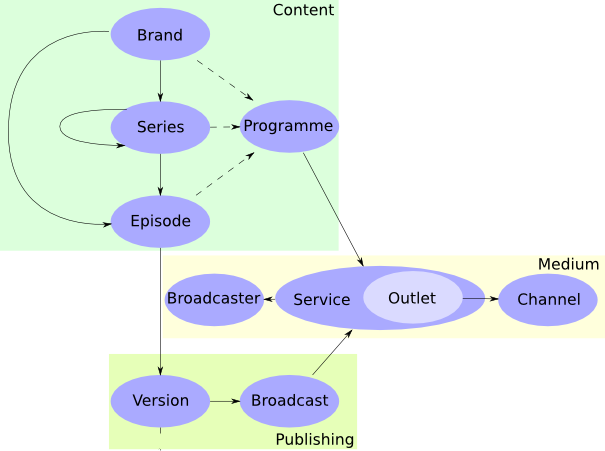
\includegraphics[width=\linewidth]{programmes_ontology.png}
\end{frame}
\note{
  We can take a quick look at different kinds of content the BBC has and why
  they present their own unique challenge.

  Here, we have the ontology that has been put together to describe
  TV and Radio programmes. Briefly, we have a brand which describes the name
  of a whole programme across all series, e.g. Doctor Who or Holby City.

  Each brand will have a number of series and each series will have a
  number of episodes. This isn't too difficult, but in terms of search, it's
  a fairly open question as to what happens if someone searches
  ``Doctor Who''. Do we present the home page for the Doctor Who programme?
  Do we offer the latest episode on iPlayer to watch on catch-up? Do we offer
  the last episode to be broadcast, even if it's an older one that was
  repeated?

  As a search application, we need to start to understand the programme data
  so we can think about how we react best to user queries.

  The data structure goes further to capture what channel it went out on
  and whether it's available to watch on a PC, on a games console such as
  Playstation 3 or on a mobile. If you search for Merlin, do you want
  the original version or the audio described for blind people? If I'm on
  a smartphone and I get search results telling me what I can watch on catch-up
  on a PC, but half of them aren't available on my phone, is that useful?

  The main point here is that programmes are what we'd call very
  \emph{structured} data. There are a lot of different kinds of objects --
  brands, series, episodes, channels, devices, etc. -- and they relate to
  each other in a very defined way. This is contrasted to, say, News which
  is more like a large body of articles, each in a single category, but
  there is little complexity on top of that.

  With structured data such as programmes, we need to think very carefully
  about how we plan to store them in the search indexes and how we plan
  for users to find that information with queries.
}

\begin{frame}
  \frametitle{How do we know if a programme is available on iPlayer?}
  \framesubtitle{7-day window}
  %TODO
  \missingfigure{}
\end{frame}
\note{
  Just to throw an extra piece of complexity in to the mix, iPlayer has
  a very specific feature in that programmes are available to watch on
  catch-up generally only 7 days after the programme aired. This means
  that just because a programme episode exists, doesn't mean someone
  can watch it on iPlayer right now. So, if someone searches for Newsnight,
  do we show them only the ones that can actually be watched or do
  we give all information on even the historic episodes no longer
  viewable? Clearly, we want to give the choice to the user, but it has
  to be considered. Currently, if you search within the iPlayer site, you can
  only find episodes that are available to watch.

  This adds an extra piece of information we need to know from iPlayer: we
  do not just want to know when a new programme is added to the database,
  but we need to know between which dates we should be telling people they
  are able to watch it on iPlayer.
}

\begin{frame}
  \frametitle{Indexing News and Sport stories}
  \framesubtitle{Rapidly-published, text content}
  %TODO
  \missingfigure{}
\end{frame}
\note{
  As mentioned, News and Sport are less structured content items in that they
  are just a collection of articles, perhaps with a date. They are
  put into categories normally, but this is still far less complex than
  iPlayer and programmes information.

  What makes them more interesting is that they will be published very quickly
  if a major story is just breaking, updated quickly if corrections are to
  be made or the story develops and perhaps even removed quickly if there
  are legal complications.

  This puts a pressure on the search application to ensure it picks up
  new, changed and removed stories very quickly and reflect those changes
  to the public as quickly as possible.

  An emerging idea around news and sport is to be able to tag them with
  topics and concepts mentioned therein. This is still not widespread on
  all articles, but it adds an extra ability for search to be able to know
  that, say, all articles relating to the Syrian civil war are related to the
  same topic. Perhaps if all articles are tagged with their topics, we could
  allow searching of concepts, topics, people and events and show the latest
  related articles rather than just searching the articles themselves? For
  example, I can search ``EU'' and get every article that mentioms the EU or
  the European Union, but perhaps if the journalists have tagged which articles
  are specifically ``about'' the EU, I can instead get a quick summary of the
  latest news about the EU.
}

\begin{frame}
  \frametitle{Indexing Children's games, Bitesize, etc.}
  %TODO
  \missingfigure{}
\end{frame}
\note{
  A lot of content for children includes games. This is an interesting
  challenge as there's no textual information other than the game's
  title. This is challenge for a tradtional web search where you're working
  with keywords found in a page of text.
}

\begin{frame}
  \frametitle{Web Crawling}
  \framesubtitle{Older pages, mothballed sites, etc.}
  %TODO
  \missingfigure{}
\end{frame}
\note{
  Whilst we would prefer to get all BBC content information directly
  from the sources, there's some cases where we still have to run a
  Google-style web crawler over our own site to find everything. There
  are a lot of sites that are simply not maintained any more that people
  may still want to find.

  One example is BBC Gardening. The site is no longer actively kept up
  to date and if we have trouble trying to get at the information, there
  is no team of employees we can contact for help. The only way we can
  present that information is to run a web crawler and just index what
  we can find.
}

% Section 11

\begin{frame}
  \frametitle{How do we search it all?}
  %TODO
  \missingfigure{}
\end{frame}
\note{
  Assuming we've got all this content indexed in the search application and
  it's being continuously updated as it should be, how do we best search it all?

  At the simplest level, we can do the usual search techniques mentioned
  earlier: we can find items that match keywords in a query. Currently,
  we break down the different ``kinds'' of content into separate zones and
  don't attempt to present a single results list as Google would, but perhaps
  we can get it down into one list? This would not be without its own problems
  however.
}

\begin{frame}
  \frametitle{Searching different types of content}
  \framesubtitle{Comparing apples and oranges}
  %TODO
  \missingfigure{}
\end{frame}
\note{
  If I search for Doctor Who, is it better to give me a news article that
  mentions that phrase a lot or the latest episode to watch on iPlayer? Given
  that the programme synopsis might only mention the phrase once and the
  news article might mention it a lot, a traditional search algorithm might
  prefer the news article. This is where we need to get clever with the deep
  knowledge we have of our own content and try to ensure the top results
  are for the right kind of thing.

  It's just a challenge when you try to mix apples and oranges like this, just
  as you couldn't tell me which was longer between a metre and a kilogram, it's
  hard to say which is more relevant between a documentary about volcanoes
  and the GCSE Geography pages that teach about them. I'm not saying we have
  all the answers right now, but it's an interesting challenge for the next
  few years.
}

% Section 12

\begin{frame}
  \frametitle{How can we keep improving the experience?}
  %TODO
  \missingfigure{}
\end{frame}
\note{
  The public aren't usually excited by a well-architected search application
  that works perfectly, so whilst it is our goal to get a lot of the
  behind-the-scenes stuff working, we will eventually be looking at how to
  make the search application a friendly, usable and useful application for
  website visitors that choose to use it.

  One important aspect of any modern web application or website is how to
  take feedback from users and provide continuous improvement to the product
  to make it better all the time. This is where web applications really
  differ from physical engineering in that you can't just sell it and
  then maintain it later, but it needs to be an evolutionary approach
  that consistently reacts to what's working and what's not, dropping the latter
  and looking to improve the former.

  To finish off, I will quickly look at how any modern web site will seek
  continuous improvement, including BBC Search.
}

\begin{frame}
  \frametitle{Analytics}
  %TODO
  \missingfigure{}
\end{frame}
\note{
  Any serious web application will be tracking analytics information about
  how the site is used and how the visitors behave. At the simplest level, we
  could track what users search for and what link they then go on to click.
  If people are always clicking result number 3 for a certain search, then
  perhaps that results number 3 actually needs to be number one?

  The example here shows a dashboard from Google's Analytics application
  for webmasters to track how their sites are used. At the BBC, have bought
  in a commercial application and don't use Google, but the principles are
  very similar.

  Overall, you're looking to track as many statistics about your visitors as
  possible and then try to see what insights you can derive from them.
  Generally, I think this is a solid starting point for doing any kind of
  improvement of your website as without stats, it's hard to say whether
  changes you make increase or reduce the users that come to you.
}

\begin{frame}
  \frametitle{Popular searches}
  %TODO
  \missingfigure{}
\end{frame}
\note{
  So, if we're tracking statistis about what people are searching, then
  perhaps we can generate a list of what are very popular searches right now.
  Some things are always popular such as popular programmes or sport teams, but
  some are popular only for a short period such as ``riots'' back when the
  riots kicked off in London and other parts of England in 2011.

  An easy improvement might be to preempt people searching for very popular
  things by providing quick links to popular items such as the Doctor Who
  homepage or News pages summarising an ongoing news event such as riots. Of
  course, we can only provide such a feature if we've used something like
  analytics to find out what those popular searches are.

  What's more difficult especially is providing popular links for events that
  have just become popular in the last few hours or even minutes. It's all
  very easy to have someone making a monthly report on what's popular in the
  long term, but a more dynamic search system would take feedback directly
  from the analytics system and start promoting or boosting things that
  appear to be popular exactly when the trend begins to happen.
}

\begin{frame}
  \frametitle{TV/Radio Broadcasts}
  %TODO
  \missingfigure{}
\end{frame}
\note{
  If you search for an older programme such as Dad's Army, maybe you are
  looking for some pages to tell you information about the programme. However,
  if BBC Two has just happened to have put out an episode on repeat last night,
  then maybe you were actually looking to watch that episode on iPlayer because
  you missed it.

  An example like this shows how BBC Search could be -- but currently isn't --
  sensitive to the TV and Radio schedules. There is a bit of a disconnect
  between the TV world and the BBC online world because we obviously work in
  very different arenas, but this is one example where sharing that information
  could be a benefit to the BBC website users.
}

\begin{frame}
  \frametitle{Responding to major events}
  %TODO
  \missingfigure{}
\end{frame}
\note{
  I mentioned this briefly when talking about analytics, but it highlighted
  a general need for the search to react when there's something big
  happening in the world or the country.

  This is not just news events such as riots or an election, but could be
  weather events such as lots of snow. When someone is searching for snow
  in the Summer, they might be looking for the educational materials
  on precipitation, but if we happen to know it's in the midst of nationwide
  reports of heavy snow and travel warnings, that people are actually looking
  to see what alerts and travel warnings there are for their area.
}

\begin{frame}
  \frametitle{Awareness of time of day...}
  \framesubtitle{... or day of the week}
  %TODO
  \missingfigure{}
\end{frame}
\note{
  Is a query for football different on a Saturday afternoon to a Monday
  morning? Are people's searches different at 10am as they are at 10pm?
  I don't really have specific answers to this right now, but time-sensitive
  searches could well be an area worth exploring.
}

\begin{frame}
  \frametitle{Location Awareness}
  %TODO
  \missingfigure{}
\end{frame}
\note{
  If I just search for ``weather'' it's a bit ambiguous as to what region's
  weather I want. Modern smartphones, web browsers, etc. allow ways for a
  user to tell a website where they are exactly and such information could
  be used to factor into a search query.

  So, if a user has previously said they are in Edinburgh and they search
  weather, I can give them Edinburgh weather. I can also give local news
  headlines if they are just looking for news. If they search for football,
  I can know to prefer Scottish leagues and the Scottish national side over
  English league articles.
}

\begin{frame}
  \frametitle{Social Media}
  Trends on Twitter, shares on Facebook
  %TODO
  \missingfigure{}
\end{frame}
\note{
  These days people like to share links to things they find interesting
  on sites such as Faceook. This is another way to tell if an items is
  particular popular. Similarly to getting stats from the analytics, can
  we feed in information dynamically from these social network sites to
  boost things in the search results we know people are very keen to read
  or watch, so much so that they then pass it on to their friends?
}

\begin{frame}
  \frametitle{The Future}
  \begin{itemize}
    \pause \item Rebuild some of the backend technology
    \pause \item Rebuild the search results pages
    \pause \item Keep finding the best ways to improve the experience for the users
  \end{itemize}
  \missingfigure{}
\end{frame}

\end{document}
